\section{Computational evidence}
\label{sec:experiments}

The recorded computations examine three consequences of the theory: the
dependence of spatial search on the tolerance and local geometry, the effect
of branching points within a fixed solver, and the separation between root
exactness and small variable-branching certificates in random designs.
They provide finite-sample comparisons of specified implementations.
The proofs in the preceding sections establish the asymptotic statements;
the computations do not establish them by extrapolation.

\subsection{Protocols and interpretation}
\label{experiments:protocols}

The spatial studies use SCIP 10.0.2 through PySCIPOpt 6.2.1, with SoPlex
8.0.2 and single-threaded solves. The recorded environment is Python
3.13.11 on Linux WSL2; the branching benchmarks identify an Intel Xeon
w5-2565X and Ipopt 3.14.19. The synthetic tolerance study does not record
the Ipopt version. Several solves ran concurrently, so timing reflects
the shared workload. We report node counts rather than time speedups.
SCIP processed nodes, final certificate leaves, and nodes of the separate
Python algorithms are different measurements.
\Cref{experiments:tab-protocols} gives the principal SCIP cohorts and
termination counts.

\begin{table}[tbp]
  \centering
  \small
  \caption{Principal SCIP cohorts and termination counts. Each count is
  a run, not a distinct instance. \texttt{optimal} and \texttt{gaplimit}
  are solver statuses; limit counts are unfinished observations. The
  120-second benchmark block contains only the core settings.}
  \label{experiments:tab-protocols}
  \begin{tabular}{@{}p{0.31\textwidth}p{0.31\textwidth}r@{}}
    \toprule
    Cohort & Protocol & Records and statuses \\
    \midrule
    Synthetic tolerance study & 20 instances; seed 0; up to 13 tolerances;
    120 s; 100,000 nodes & 2,134 total \\
    & & 1,655 gap limit \\
    & & 420 optimal; 59 node limit \\
    \addlinespace
    Branching benchmark, first campaign & 57 instances; 5 settings;
    3 seeds; 120 CPU s & 855 total \\
    & & 797 optimal \\
    & & 57 time limit; 1 crash \\
    \addlinespace
    Branching benchmark, second campaign & 57 instances; 12 settings;
    3 seeds; 60 CPU s & 2,052 total \\
    & & 1,943 optimal \\
    & & 104 time limit; 5 crashes \\
    \addlinespace
    Synthetic kink study & 16 instances; 12 settings; 5 seeds;
    4 tolerances; 60 s & 3,840 total \\
    & & 2,024 gap limit; 1,816 optimal \\
    \bottomrule
  \end{tabular}
\end{table}


An \texttt{optimal} status denotes exhaustion of the solver's search under
its numerical tests. A \texttt{gaplimit} status denotes its global gap
stopping test. Neither status is an exact-arithmetic certificate of the
mathematical optimum. In the tolerance study, \texttt{limits/absgap} is set
to $\epsilon$ and the relative-gap limit to zero; $\epsilon$ is not a slack
added to every node-pruning test. Feasibility tolerance is $10^{-9}$,
whereas the requested gaps range from $10^{-1}$ to $10^{-7}$ in half-decade
steps. Recorded incumbents can lie as much as $5.5\times10^{-9}$ below the
known mathematical optimum because of accepted constraint violations.
Some LP tolerance requests were also refused by SoPlex. These distinctions
matter when comparing the solver with a theorem that assumes valid lower
bounds and an exact incumbent.

The accompanying computational archive preserves the original generation
and analysis code, run records, metadata, selected-instance lists, and
numerical summaries. An inventory records source paths, byte counts, and
SHA256 hashes; figure metadata identify every plotted observation and its
original record. The package checks accounting and aggregation without
invoking a solver. Such checks establish the integrity of the retained
evidence, rather than the mathematical validity of floating-point bounds.
External MINLPLib model files and solver binaries are not included.

\subsection{Tolerance, geometry, and solver representation}
\label{experiments:tolerance}

The tolerance study contains 20 synthetic instances with optima known by
construction. It uses epigraph formulations $\min t$ subject to
$f(x)\leq t$ and the instance constraints, with fixed expression forms.
Each run has a 100,000-node limit and a 120-second limit; a tolerance
sequence stops after its first limit. The setting named \texttt{model}
supplies the known optimum as incumbent, disables heuristics, and uses
best-first node selection without plunging. Ordinary propagation remains
enabled. These three changes were made together, so their individual
effects are not identified by a comparison with the default setting.

The main unconstrained families are built from
\[
 h_c(s)=(s-1)^2\big((s+1)^2+c\big),\qquad
 q_d(s)=(s+d)^4+(s-d)^4-12d^2s^2-2d^4=2s^4.
\]
The isolated \texttt{iso}$n$ objectives sum $h_{c_i}(x_i)$, with
$(c_1,c_2,c_3,c_4)=(0.5,0.7,0.6,0.8)$; \texttt{iso2c} adds
$0.5(x_1-x_2)^4$. The objectives for \texttt{linediag2} and
\texttt{plane3} are $h_{0.5}(x_1-x_2)$ and
$h_{0.5}(x_1+x_2-x_3)$. The axis-aligned \texttt{lineaxis2} adds
the unsimplified zero $q_{0.375}(x_2)-2x_2^4$ to $h_{0.5}(x_1)$.
The \texttt{ring2} and \texttt{sphere3} objectives are
$(\sum_i x_i^2-1)^2$ in two and three dimensions.
The quartic objectives \texttt{qflat1}, \texttt{qflat2a},
\texttt{qflat2b}, and \texttt{qflat3} respectively use $q_{0.375}(x_1)$,
$h_{0.5}(x_1)+q_{0.375}(x_2)$,
$q_{0.375}(x_1)+q_{0.5}(x_2)$, and
$h_{0.5}(x_1)+q_{0.375}(x_2)+q_{0.5}(x_3)$.
These expressions are passed in the stated expanded or unsimplified
forms, not replaced by their algebraically simpler identities.
The exponential examples minimize $\log x_2-x_1$ subject to
$x_2\geq e^{x_1}$, or the sum of two such independent copies.
The two McCormick examples minimize
$2|d| - d(x_2-b)$ on $[0,1]^2$, with $b=\sqrt2-1$ and
$d=x_1-1/3$ (aligned) or $d=x_1-x_2-1/3$ (transversal).
The archive supplies all coordinate bounds, which are asymmetric in the
non-McCormick examples, and the generated solver formulations.

\begin{figure}[tbp]
  \centering
  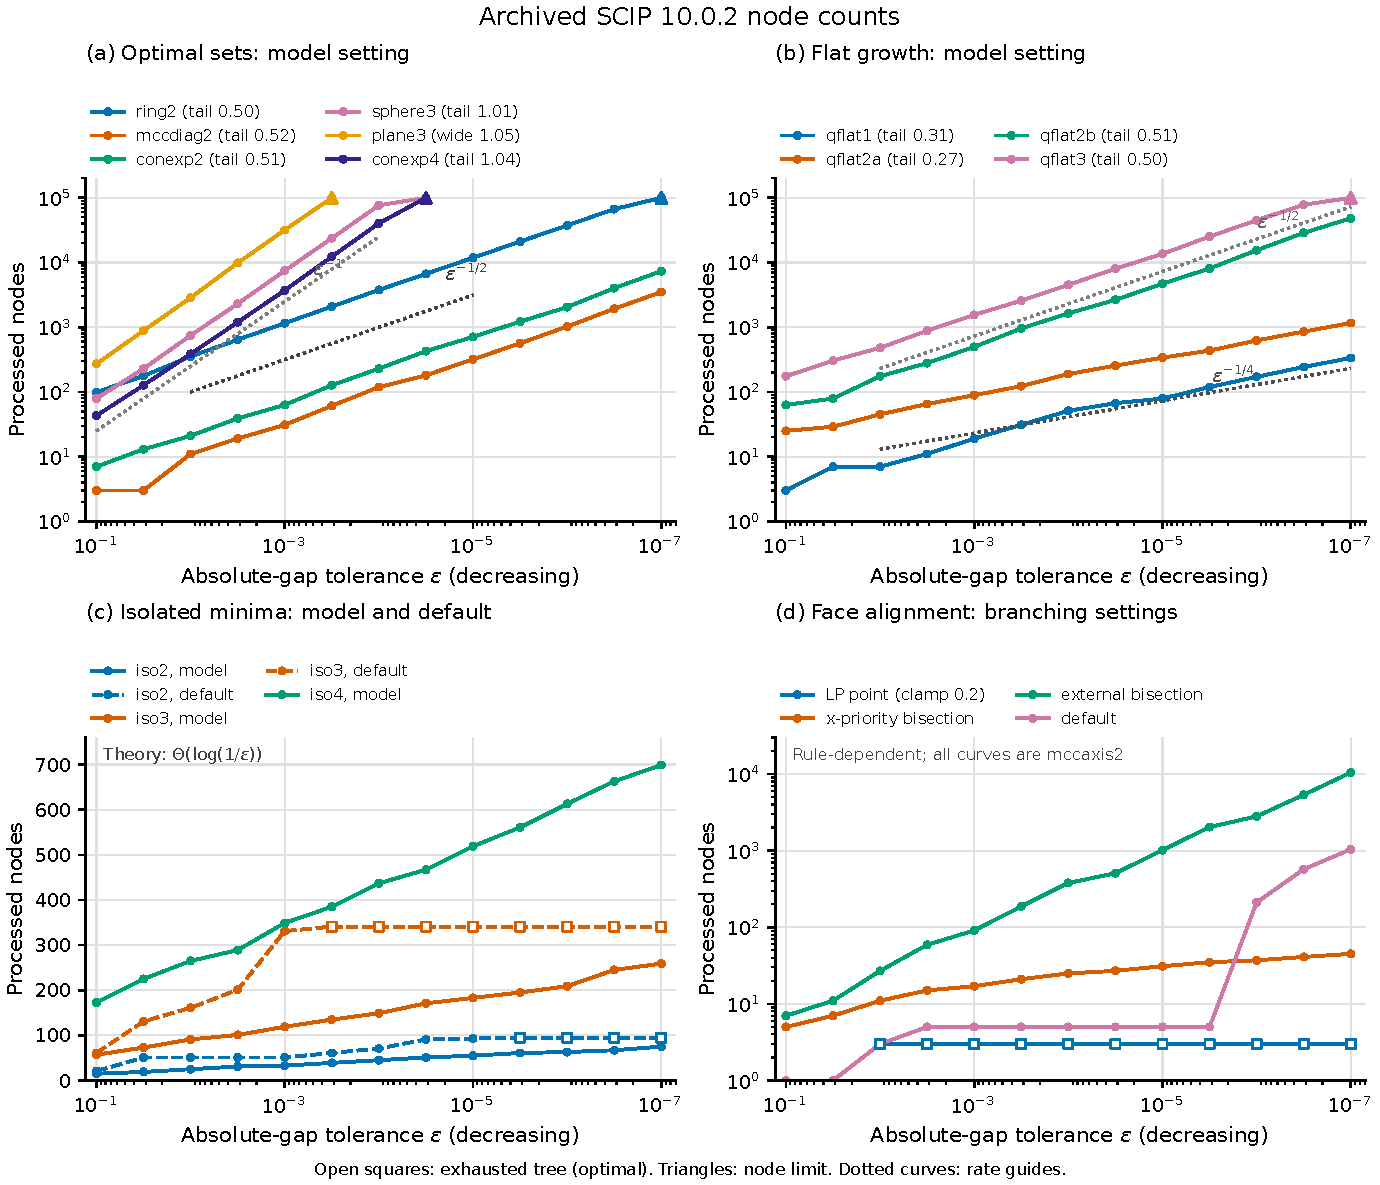
\includegraphics[width=\textwidth]{figures/node-scaling.pdf}
  \caption{Recorded SCIP 10.0.2 processed-node counts: 230 observations in
  19 separate instance/setting curves, covering 14 of the tolerance study's
  20 instances. Panels (a) and (b) use \texttt{model}: optimal incumbent,
  heuristics disabled, best-first selection, ordinary propagation enabled.
  Dotted guides are arbitrarily normalized theorem powers, not absolute
  predictions. Legend slopes are the archived finite-window fits described
  in the text. Panel (c) has a linear node axis to show additive growth and
  default-solver saturation; default \texttt{iso4} is omitted for legibility
  (3,431 nodes at $10^{-7}$). Panel (d) compares branching settings on an
  aligned McCormick instance. External bisection and its $x_1$-priority
  variant use best-first search with propagation, heuristics, and presolve
  disabled; LP-point and default settings use ordinary search. Tolerance
  axes are logarithmic and decrease to the right; other node axes are
  logarithmic. Open squares mark exhausted trees; triangles mark counts at
  the node limit. No observations are pooled or averaged. The requested
  absolute gap is a global stopping test, and these floating-point counts
  are not rigorous $\epsilon$-certificates.}
  \label{experiments:fig-scaling}
\end{figure}

\Cref{experiments:fig-scaling}(a) shows the predicted $1/2$ and $1$
exponent groups. For the line and sphere families with quadratic
transverse growth, \Cref{sec:geometry} predicts power $p/2$ for a
$p$-dimensional optimal set. The constrained and McCormick examples
additionally depend on their specific gap structure.
Under \texttt{model}, the families with one-dimensional optimal sets have fitted slopes
$0.50$--$0.52$, compared with the predicted exponent $1/2$; the
families with two-dimensional optimal sets have slopes $1.01$--$1.05$, compared with $1$.
The latter fits span only one or two decades; their available sequences
cover two or three decades before the node budget limits further
observations. For example, \texttt{sphere3} has 79, 747,
7,475, and 76,699 processed nodes at tolerances $10^{-1}$ through
$10^{-4}$. These observations support the geometric distinction in
\Cref{sec:geometry}, within the tested formulations and search settings.

Degenerate isolated minima also show why dimension alone is insufficient.
For local growth $\sum_i |t_i|^{q_i}$, the predicted power is
$n/2-\sum_i1/q_i$. The quartic examples \texttt{qflat2b} and
\texttt{qflat3} give fitted powers $0.49$--$0.51$, compared with $1/2$.
For \texttt{qflat2a}, the predicted power is $1/4$ and the
\texttt{model} tail fit is $0.27$. The one-dimensional quartic
\texttt{qflat1} has tail and wide fits $0.31$ and $0.33$ under
\texttt{model}, while controlled bisection gives $0.25$ and $0.24$.
The records do not determine whether the discrepancy under LP-biased
branching persists or reflects the finite tolerance window.

At isolated nondegenerate minima, \texttt{model} counts grow
approximately additively with $\log(1/\epsilon)$: the archived fits give
9, 10, 40, and 92 nodes per decade for \texttt{iso2}, \texttt{iso2c},
\texttt{iso3}, and \texttt{iso4}. The default counts for
\texttt{iso2} and \texttt{iso3} instead plateau at 95 and 341 nodes.
Those runs exhaust their trees near the numerical feasibility scale.
Their plateaus therefore do not establish tolerance-independent
mathematical certificate sizes.

The archived slopes are least-squares fits of $\log_{10}$ nodes against
$\log_{10}(1/\epsilon)$. A tail fit uses the last five available eligible
records with $\epsilon\leq10^{-3}$; a wide fit uses all eligible records
with $\epsilon\leq10^{-2}$. Both require at least three points spanning
0.99 decades. Node-limit, time-limit, and error records are excluded,
whereas exhausted trees remain eligible. A short fit or an exhausted-tree
plateau can therefore differ substantially from an asymptotic exponent.
Limits also truncate the harder sequences, so the slopes describe the
observed range rather than an uncensored distribution of solver work.

For seven instances satisfying the archived integral-bound hypotheses,
recorded final leaves, including leaves still open at gap termination,
were compared with the anisotropic integral lower bound. No recorded ratio
is below one; the smallest is $1.59$ on \texttt{qflat1}. Under
\texttt{model}, the leaf-to-bound ratio ranges from $6.84$ to $9.78$
on \texttt{iso2}, $15.88$ to $23.65$ on \texttt{linediag2}, and
$6.76$ to $9.41$ on \texttt{qflat2a}. The last range includes every
eligible half-decade observation. This is a consistency check on recorded
leaves and numerically evaluated bounds, not a certified inequality for
the floating-point run.

Expression representation can change the effective relaxation. On
\texttt{ring2}, keeping an outer square unexpanded gives one processed
node at every tested tolerance, whereas \texttt{model} with the expanded
expression uses 37,439 nodes at $10^{-6}$. Shared auxiliary expressions
likewise produce one-node runs on \texttt{condisk2}. Objective-cutoff
propagation gives 15 nodes over $10^{-2}$ through $10^{-7}$ on
\texttt{isofbbt2}, whose fourth-order secant gap lies outside the quadratic
gap hypothesis. These examples concern changes to the relaxation and its
propagation, as in \Cref{sec:propagation}; they do not contradict lower
bounds for a fixed oracle satisfying that hypothesis.

Face alignment produces a different branching effect. On the aligned
McCormick instance \texttt{mccaxis2} at $\epsilon=10^{-7}$, LP-point
branching uses 3 nodes, external bisection restricted to $x_1$ uses 45,
and external bisection on both variables uses 10,469. The external
bisection runs disable presolve and propagation and use best-first search,
so the comparison identifies attainable regimes rather than isolating a
single parameter. Its bounded, logarithmic, and power-like sequences
illustrate the McCormick mechanism of \Cref{sec:geometry}. The transversal
instance \texttt{mccdiag2} has no bounded sequence among the tested
settings. For these tests SCIP's variable-lock reduction is disabled:
with that reduction, \texttt{mccaxis2} becomes binary in one variable and
is solved at the root, changing the permitted operations.

\subsection{Branching points on a selected benchmark}
\label{experiments:benchmark}

The MINLPLib benchmark consists of 57 nonconvex instances selected by a
default-solver screen, subject to size filters and a cap of three instances
per family. Screened default solution times lie between 1 and 20 seconds;
24 instances have integer variables, and five perform no continuous
branching. This is a selected, relatively short-running benchmark rather
than a sample of all nonconvex problems. The two campaigns use the same
instance names but different limits and settings. The first campaign has
855 core runs, $57\times5\times3$, at 120 CPU seconds. Its 171 optional,
228 tolerance-sweep, 486 screening, and 187 diagnostic records are separate
from the core comparison; together all batches total 1,927 records.
The second campaign has $57\times12\times3=2,052$ runs at 60 CPU seconds.
Both use default numerical tolerances and zero requested absolute and
relative gaps. We retain these campaigns as separate measurements.

Within each campaign, seed labels 0, 1, and 2 are matched across settings;
the latter two change SCIP's variable permutation and random-seed shift.
The instance is the statistical unit. If $n_{isk}$ is the observed count
for instance $i$, setting $s$, and seed $k$, define
\[
  g_{is}=\exp\left\{\frac{1}{|K_{is}|}
                  \sum_{k\in K_{is}}\log(n_{isk}+10)\right\}.
\]
For a setting $s$ and reference $r$, the reported ratio is
\begin{equation}
  R_{s/r}=\exp\left\{\frac{1}{|I|}
                \sum_{i\in I}\log\frac{g_{is}}{g_{ir}}\right\}.
  \label{experiments:eq-ratio}
\end{equation}
Thus the shift is 10 nodes, and large instances do not dominate by their
absolute counts. Intervals use 5,000 bootstrap resamples of paired
instances, with bootstrap seed 1; they do not treat the three seed runs as
independent benchmark instances. Reported $p$-values use a two-sided
Wilcoxon signed-rank normal approximation on per-instance log ratios.
They are unadjusted for the multiple comparisons.

Time-limited runs enter with their count at termination, which can
understate completed-tree work. Crashes are handled as in the original
analyses: the first campaign averages the available seed counts for that
setting, whereas the second omits a paired instance if any required count
is missing. \Cref{experiments:tab-branching} reports the resulting paired
cohort sizes and the full per-setting termination counts.

\begin{table}[tbp]
  \centering
  \small
  \caption{Separate MINLPLib branching comparisons. Ratios use shift 10
  and \eqref{experiments:eq-ratio}; intervals are paired-instance
  bootstrap intervals. $m$ is the number of instances contributing node
  ratios. Termination counts cover all 171 runs of the row's setting,
  including any instance omitted from a paired ratio. O/T/C denote
  \texttt{optimal}, time limit, and crash.}
  \label{experiments:tab-branching}
  \begin{tabular}{@{}llrrlr@{}}
    \toprule
    Setting & Reference & $m$ & Ratio & 95\% interval & O/T/C (of 171) \\
    \midrule
    \multicolumn{6}{@{}l}{First campaign: 120 CPU s; SCIP selection} \\
    \texttt{default} & -- & -- & 1 & -- & 170/1/0 \\
    \texttt{lp} & \texttt{default} & 57 & 1.03 & $[0.83,1.26]$ & 166/5/0 \\
    \texttt{lp\_noclamp} & \texttt{default} & 57 & 2.18 & $[1.43,3.39]$ & 138/32/1 \\
    \texttt{mix\_noclamp} & \texttt{default} & 57 & 1.35 & $[1.03,1.85]$ & 154/17/0 \\
    \texttt{mid} & \texttt{default} & 57 & 1.15 & $[1.03,1.28]$ & 169/2/0 \\
    \addlinespace
    \multicolumn{6}{@{}l}{Second campaign: 60 CPU s; \texttt{x\_} settings use the plugin} \\
    \texttt{default} & -- & -- & 1 & -- & 168/3/0 \\
    \texttt{rclamp} & \texttt{default} & 56 & 0.96 & $[0.87,1.06]$ & 170/0/1 \\
    \texttt{lp} & \texttt{default} & 57 & 1.01 & $[0.81,1.21]$ & 163/8/0 \\
    \texttt{x\_lp} & -- & -- & -- & -- & 164/7/0 \\
    \texttt{x\_recenter} & \texttt{x\_lp} & 56 & 0.94 & $[0.86,1.01]$ & 162/8/1 \\
    \texttt{x\_recenter} & \texttt{default} & 56 & 0.92 & $[0.71,1.14]$ & 162/8/1 \\
    \texttt{x\_noclamp} & \texttt{x\_lp} & 56 & 2.00 & $[1.43,2.96]$ & 129/41/1 \\
    \bottomrule
  \end{tabular}
\end{table}


SCIP's default point rule combines a relaxation point with midpoint pull
0.75, a relative-width trigger of 0.5, and clamp 0.2 away from the variable
bounds. The first campaign compares
this rule with zero midpoint pull (\texttt{lp}), zero pull and zero clamp
(\texttt{lp\_noclamp}), default pull with zero clamp
(\texttt{mix\_noclamp}), and pure midpoint splitting (\texttt{mid}).
The LP-point ratio is $1.03$ with interval $[0.83,1.26]$, so this benchmark
does not resolve an aggregate improvement. Pure midpoint splitting gives
$1.15$ with interval $[1.03,1.28]$ and $p=0.009$.
Seed variability is substantial: among the 56 instances with three
completed default runs, the median ratio of largest to smallest shifted
node count is $1.51$.

Clamp removal gives ratio $2.18$ with interval $[1.43,3.39]$ and 33 of
171 runs without an \texttt{optimal} termination, including one crash.
The retained diagnostics identify a concrete mechanism: on 10 of the
16 instances with an LP/no-clamp failure, the branching variable's LP
value lies on a bound in 42--100\% of the bounded continuous branchings.
Without the clamp, the split lies only at the solver's numerical offset
from that bound and can create long chains of nearly unchanged boxes.
Restricting the comparison to instances where all runs of both settings
finish gives ratio $1.08$ on 41 instances. That restriction removes much
of the observed failure penalty and changes the question being measured.

The second campaign has two arms. Parameter-only settings use SCIP's
selection; settings prefixed \texttt{x\_} use an external-branching plugin
with a closely related selection rule. The plugin implements clipping,
randomized clamping, recentring, and an incumbent-coordinate rule.
Its selection and the point-formula inspection use SCIP 10.0.3 source,
whereas the recorded executable is 10.0.2; the arms should therefore not
be treated as an exact reproduction of one another.
The randomized clamp ranges over $[0.1,0.3]$, and recentring uses
safeguard parameter 0.2.
Recentring gives $0.94$ against the plugin LP-point rule and $0.92$ against
SCIP's default, with intervals containing one. Randomized clamping also
has an interval containing one. Removing the plugin clamp gives $2.00$
with interval $[1.43,2.96]$ and 41 time limits. The two campaigns therefore
agree on the boundary-chain failure mechanism, while providing no
resolved general gain from the safe variants.

The second campaign also contains 3,840 synthetic kink runs: two families,
eight kink positions, twelve settings, five seeds, and four tolerances
$10^{-2},10^{-4},10^{-6},10^{-8}$. These runs supply the optimum and disable
heuristics, propagation, and weak-dual cutoff reductions, which would
otherwise solve the one-dimensional kink at the root; feasibility
tolerance is $10^{-9}$. For the
one-dimensional kink at $a=1/6$, LP-point clipping with clamp $0.2$ uses
3, 7, 9, and 13 nodes over those tolerances, whereas the plugin recentring
rule uses 5 throughout. At $10^{-8}$ on the McCormick kink with the same
position, the ordinary LP/clipped rule averages 7,190 nodes and plugin
recentring averages 21 over five seeds. These examples expose the trap
mechanism in \Cref{sec:branching}; they do not imply the same improvement
with ordinary propagation or on the selected benchmark. Randomized
clamping also has a wide finite-sample spread: at a McCormick kink near
$a=0.0102$, its ordinary LP-point variant averages 766 nodes, with range
7--3,443, versus 26 with the fixed clamp. Independent exact rational
model records, kept separate from SCIP, give 19,537 processed model nodes for
widest-side clipping at $a=1/6$, clamp $1/5$, and $\epsilon=10^{-8}$.

\subsection{Finite-size certificates in random designs}
\label{experiments:random}

The random-design studies use their own Python node algorithms and
Gaussian instance generators. The recorded stack is Python 3.13, NumPy
2.5, SciPy 1.18, and Clarabel 0.11; semidefinite comparisons additionally
use CVXPY and, for larger sparse problems, SCS. Node decisions evaluate
explicit dual bounds or Frank--Wolfe lower bounds rather than accept a
solver's reported objective alone. These formulas give a mathematical
certificate when evaluated with controlled error; the archived
evaluations are floating point. We therefore describe their recorded
certificate decisions without treating them as interval-validated proofs.

For sparse regression, the main finite-size comparison has Gaussian
design $X$, $k=8$ planted coefficients of magnitude $b=1$, per-entry noise
standard deviation $\sigma=0.5$, and
\[
 n=\operatorname{round}(\alpha k\log p),\qquad
 \lambda=1.5\sigma\sqrt{2n\log p}/b.
\]
Eight independent design/noise seeds are used in each cell; varying
parameters on a shared seed does not produce independent new instances.
The perspective lower bounds test the planted-support value, and a root
certificate is the sufficient planted-point certificate discussed in
\Cref{sec:regression}. C1 tests every single wrong fixing against that
value. When it holds, its certificate also establishes planted optimality
under the assumptions of that section. A failing wrong-fixing relaxation
does not by itself show that a better integer support exists.

\begin{table}[tbp]
  \centering
  \small
  \caption{Recorded finite-sample C1 passes, with denominators.
  (a) Sparse regression: $k=8$, $b=1$, $\sigma=0.5$, the scaled ridge
  rule in the text, and eight independent design/noise seeds per cell.
  The $\alpha$ values are nominal; the displayed $n$ includes rounding.
  All eight planted-point root tests fail in each of these eight cells.
  (b) Binary least squares: square systems ($\beta=1$),
  $\theta=\rho/N$, and the archived C1 decision tests. A dash means no
  recorded cell, not a failed test. Failed C1 tests do not prove large
  trees.}
  \label{experiments:tab-finite-c1}
  \begin{tabular}{@{}rrrrr@{}}
    \toprule
    \multicolumn{5}{@{}l}{(a) Sparse regression} \\
    $p$ & $n$ at $\alpha=1.5$ & C1 & $n$ at $\alpha=1.75$ & C1 \\
    \midrule
    100  & 55 & $8/8$ & 64  & $8/8$ \\
    200  & 64 & $8/8$ & 74  & $8/8$ \\
    400  & 72 & $6/8$ & 84  & $8/8$ \\
    1,600 & 89 & $7/8$ & 103 & $8/8$ \\
    \bottomrule
  \end{tabular}

  \medskip
  \begin{tabular}{@{}rrrr@{}}
    \toprule
    \multicolumn{4}{@{}l}{(b) Binary least squares} \\
    $N$ & C1 at $\theta=0.25$ & C1 at $\theta=0.40$ & C1 at $\theta=0.50$ \\
    \midrule
    100 & $0/8$ & -- & $5/8$ \\
    200 & $0/8$ & -- & $4/8$ \\
    400 & $0/6$ & -- & $6/6$ \\
    800 & -- & $2/4$ & $4/4$ \\
    \bottomrule
  \end{tabular}
\end{table}


\Cref{experiments:tab-finite-c1}(a) shows a finite-size window with many
C1 passes and no planted-point root certificate in the displayed cells.
At nominal $\alpha=1.75$, all eight instances pass C1 at every displayed
$p$, while none passes the root criterion. This illustrates the
distinction between a linear variable-branching certificate and an exact
root relaxation. It does not measure the asymptotic constants of
\Cref{sec:regression}: the computations have $p\leq3,200$ and small $k$,
outside the proved condition $(\log p)^6\leq n\leq p$. In the revised
records, 31 earlier undecided C1 cases were
resolved, with 30 passes and one failure; the displayed decisions use those
revised records.

The separate rule comparison contains 72 instances at $p=100$ and $200$.
In three, every single deletion of a planted variable is prunable while
full C1 fails because of forced-in null variables. On these three instances,
largest-$z$ branching uses 13, 13, and 17 nodes, and most-fractional
branching uses 23, 17, and 23. The removal half of C1 and full C1 must
therefore be distinguished, as must these two branching rules. The
observations show small trees in both rules in these cases; they do not
identify an asymptotic rule-dependent window.

The stronger sparse-relaxation comparison is a separate experiment:
$k=3$, $b=1$, $\sigma=0.5$, nested columns on a shared design per seed,
and $\lambda=1.5\sigma\sqrt{2n\log 200}/b$ fixed as $p$ varies.
With $n=20$, the median fraction of the perspective root gap, measured
relative to the numerically enumerated global optimum, closed by the
optimal-perspective semidefinite relaxation is 51\%, 25\%, 12\%, and 3\%
at $p=40,80,160,320$, respectively. Eight seeds are recorded per cell;
the fractions use the seven, eight, eight, and eight runs, respectively,
whose relative perspective root gap exceeds $10^{-4}$.
For $n=40$
and $p=3,200$, the retained comparison uses the six of eight instances
where C1 establishes planted optimality. Explicit feasible lifted points
give a strictly better value than the planted point for the pairwise hull
in four of those six. The relevant lift retains helper columns whose
selectors are zero, as in the hard-side model in \Cref{sec:regression}. This selected
finite-size example illustrates the helper-column mechanism; it neither
estimates its asymptotic threshold nor establishes the exactness of a
different stronger relaxation on the full instance.

For binary least squares, the generator is
$y=\sqrt{\rho/N}\,H x^*+w$, with $M=\beta N$ rows, standard Gaussian
$H$ and $w$ independent, and $x^*\in\{-1,1\}^N$. Node bounds use the box relaxation, and
best-first search is supplied with $x^*$ as incumbent.
The C1 archive has 330 decisions, all labelled certified or refuted by
the archived bound and feasible-point tests.
\Cref{experiments:tab-finite-c1}(b) displays square-system cells without
interpolating missing parameter values. At these sizes the transition
cells lie near $\rho/N=0.4$--$0.5$, above the limiting C1 constant $1/4$
in \Cref{sec:binary-least-squares}. Tall-system cells with $\beta=2$
move from about $0.12$--$0.17$ at $N\leq400$ toward $0.10$--$0.12$ at
$N=800$, compared with the limiting constant $1/12$.
These are small-sample frequencies of a sufficient condition. C1 failure
does not establish a lower bound above linear on every search tree.

The tiny-system root study uses 20,000 trials per cell for
$N\in\{2,4,6,8\}$, $\beta\in\{1,2\}$, and
$\rho\in\{1,4,16,64\}$.
The observed frequency that the planted $x^*$ minimizes the box relaxation
is close to $2^{-N}$. The event that some binary vertex minimizes that
relaxation is different and can have a larger frequency. Neither event
should be identified with successful rounding of a fractional solution.
In square systems with $\rho=4\log N$, the geometric-mean
most-fractional node counts are 44, 97, 509, and 15,765 at
$N=32,64,128,256$, from six, six, six, and four seeds, respectively.
The static-order trees at $N=256$ hit the 100,000-node budget in all
four runs; those records are lower observations of work, not completed
tree sizes. The rapid finite-size growth is consistent with a difficult
box-certificate regime, but proves no growth law. In particular, the
explicit hard-regime lower-bound constants are too small to give a useful
numerical bound at the tested dimensions.

The benchmark intervals describe the selected instances and paired seed
runs; the random-design frequencies describe their stated finite cells.
Neither provides a universal branching recommendation or a practical
speedup guarantee.
